
\section{Data Fusion} \label{data_fus}

%http://www.slideshare.net/paveenju/2014-data-fusionpptx
%https://books.google.pt/books?id=6Im9BwAAQBAJ&pg=SA1-PA7&lpg=SA1-PA7&dq=data+fusion+identity+declaration&source=bl&ots=lyTWUcUAlk&sig=LhmwoIGX2SmVMMNR-OQ6exRIu1c&hl=pt-PT&sa=X&ved=0ahUKEwj6qpiI_4TRAhWEWhQKHQRmA-4Q6AEIKTAB#v=onepage&q&f=false 1-7

Data fusion is a process of combining data from different sources to improve the performance of prediction models. It deals with association, detection, correlation and estimation of data to achieve a better information of the system's state. In the fusion process, data is collected by $ N $ different source types (e.g. \gls{ir} and \gls{uv} data). The data can then be pre-processed to extract a feature vector that represents the observed data, and a machine learning approach, using the observed objects, may be performed. The output of this process must be partitioned into groups representing observations belonging to the same category and, finally, the fusion algorithms combine the multi-source data to obtain a result that has less uncertainty than it would if these sources were used individually. 

There are three main categories of data fusion, depending on the abstraction level the fusion of identity declarations takes place: \gls{llf}, \gls{ilf} and \gls{hlf}. A graphical representation of these approaches is shown in \autoref{data_fusion}.


\begin{figure}[!htb]
	\centering
	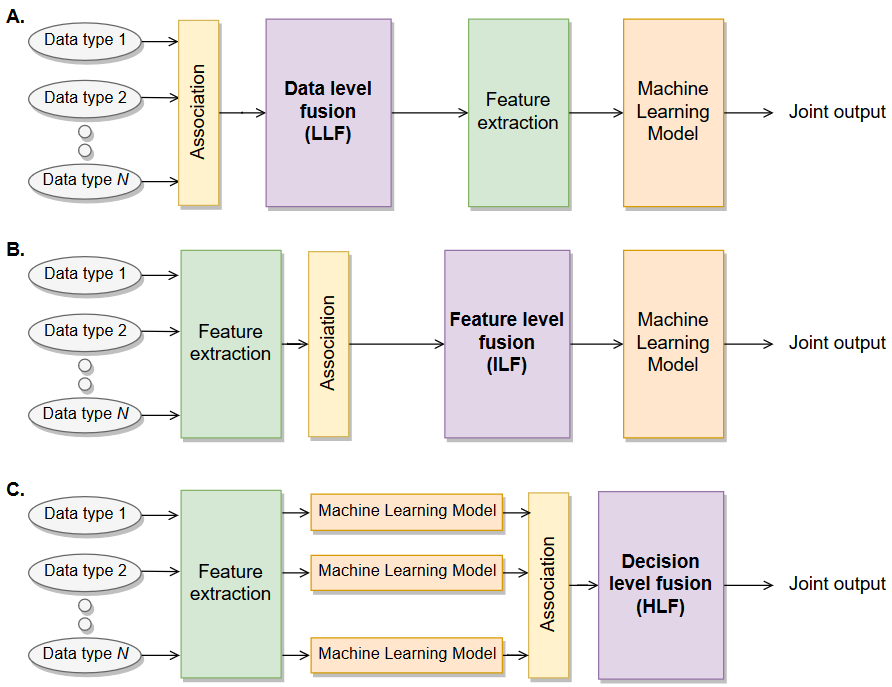
\includegraphics[width=1\linewidth]{Imagens/data_fusion}
	\caption{Graphical representation of \textbf{A.} \acrfull{llf}, \textbf{B.} \acrfull{ilf} and \textbf{C.} \acrfull{hlf}.}
	\label{data_fusion}
\end{figure}


\gls{llf} is made on a data level, by direct association and combination of raw data, representing measures of the same physical phenomena. After data combination, a feature vector is extracted and used in a machine learning process. It provides the most accurate results, assuming proper data association.

\gls{ilf} on the other hand is made on a feature level. Here, a representative features vector is extracted directly from the data. After data alignment and association, the feature vectors are concatenated into a single vector acting as an input for a machine learning process. The output is, therefore, based on the combined feature vectors from all of the data types.

Lastly, \gls{hlf} is made on a decision level. Initially, the data from each of the data types are used in a machine learning process, which can be coupled with feature extraction (e.g. using neural networks). Data association and correlation are still required to ensure that the data to be fused refer to the same physical entity. Finally, the the results from the machine learning process using each of the data types are combined using decision level fusion techniques (e.g. Bayesian inference) \citep{fourati2015multisensor}.

\gls{llf} and \gls{ilf} approaches were applied for instance in the classification of pure and adulterated honey \citep{norazian2012hybrid}. Combining e-nose and \gls{ir} data they found these two approaches achieved better results than single modality data. An \gls{hlf} approach using Bayesian inference was applied in the discrimination of white grape varieties (\gls{ftir} and \gls{uv} data), having achieved half the misclassification error when compared to the use of single modality data \citep{roussel2003fusion}.





